\documentclass{article}
\usepackage{amsmath}
\usepackage{amssymb}
\usepackage{braket} % For \ket and \bra notation
\usepackage{tikz}

% 1. Add the biblatex package and choose your style (e.g., numeric)
\usepackage[style=numeric, sorting=none]{biblatex}

% 2. Tell LaTeX where your bibliography file is located
\addbibresource{references.bib}


\newtheorem{theorem}{Theorem}[section]
% To match the specific numbering (4.1), you can manually set the section counter if needed:
% \setcounter{section}{4}

\begin{document}


% --- YOUR BODY TEXT ---

\noindent The following theorem and its proof (copied and a few details added) is stated in Camps et al.~\cite{camps2024explicit}. They say it is a variant of [Gilyén et al., 2019, Lemma 48 (in the full version)]. It asserts that such a sparse matrix can be block encoded if we can construct unitaries that can encode both the nonzero structure (the positions of the nonzero elements) and the nonzero values of the matrix A.

\setcounter{section}{4} % Sets section to 4 so theorem is 4.1
\begin{theorem}
Let $r_{\ell j}$ be the row index of the $\ell$th (among a list of $s$) non-zero matrix elements in the $j$th column of an $s$-sparse matrix $A \in \mathbb{C}^{N \times N}$ with $N = 2^n$, where $s = 2^m$. If there exists a unitary $O_r$ such that
\begin{equation}
O_r \ket{\ell} \ket{j} = \ket{\ell} \ket{r(j, \ell)},
\end{equation}
and a unitary $O_A$ such that
\begin{equation}
O_A \ket{0} \ket{\ell} \ket{j} = \left( A_{r(j,\ell), j} \ket{0} + \sqrt{1 - |A_{r(j,\ell), j}|^2} \ket{1} \right) \ket{\ell} \ket{j},
\end{equation}
then
\begin{equation}
U_A = (I_2 \otimes D_s \otimes I_N) (I_2 \otimes O_r) O_A (I_2 \otimes D_s \otimes I_N),
\end{equation}
block encodes $A/s$. Here $D_s$ is called a diffusion operator and is defined as
\begin{equation}
D_s = \underbrace{H \otimes H \otimes \cdots \otimes H}_{m},
\end{equation}
\end{theorem}

\noindent \textit{Proof.} Note that applying $D_s$ to $\ket{0^m}$ yields
\begin{equation*}
D_s \ket{0^m} = \frac{1}{\sqrt{s}} \sum_{\ell=0}^{s-1} \ket{\ell},
\end{equation*}
where $\{\ket{\ell}\}$ forms the computational basis in the Hilbert space defined by $m$ qubits. Our goal is to show that $\bra{0} \bra{0^m} \bra{i} U_A \ket{0} \ket{0^m} \ket{j} = A_{ij}/s$. In order to compute the inner product $\bra{0} \bra{0^m} \bra{i} U_A \ket{0} \ket{0^m} \ket{j}$, we apply $D_s, O_A, O_c$ to $\ket{0} \ket{0^m} \ket{j}$ successively as illustrated below
\begin{align}
\ket{0} \ket{0^m} \ket{j} &\xrightarrow{D_s} \frac{1}{\sqrt{s}} \sum_{\ell \in [s]} \ket{0} \ket{\ell} \ket{j} \nonumber \\
&\xrightarrow{O_A} \frac{1}{\sqrt{s}} \sum_{\ell \in [s]} \left( A_{r(j,\ell), j} \ket{0} + \sqrt{1 - |A_{r(j,\ell), j}|^2} \ket{1} \right) \ket{\ell} \ket{j} \label{eq:successive_application} \\
&\xrightarrow{I \otimes O_c} \frac{1}{\sqrt{s}} \sum_{\ell \in [s]} \left( A_{r(j,\ell), j} \ket{0} + \sqrt{1 - |A_{r(j,\ell), j}|^2} \ket{1} \right) \ket{\ell} \ket{c(j,\ell)}, \nonumber
\end{align}

where $[s]$ denotes the set of integers $\{0, 1, \dots, s - 1\}$. Instead of multiplying the leftmost factor $I_2 \otimes D_s \otimes I_N$ in (4.4) to last line of (4.6), we apply it to $\ket{0}\ket{0^m}\ket{i}$ first to obtain
\begin{equation}
\ket{0}\ket{0^m}\ket{i} \xrightarrow{D_s} \frac{1}{\sqrt{s}} \sum_{\ell' \in [s]} \ket{0}\ket{\ell'}\ket{i}.
\end{equation}

Finally, taking the inner product between (4.6) and (4.7) yields
\begin{align}
& \bra{0}\bra{0^m}\bra{i} U_A \ket{0}\ket{0^m}\ket{j} \\
& = \frac{1}{\sqrt{s}} \sum_{\ell'} \bra{0}\bra{\ell'}\bra{i} \frac{1}{\sqrt{s}} \sum_{\ell} \left( A_{c(j,\ell),j} \ket{0} + \dots \right) \ket{\ell}\ket{c(j,\ell)} \\
& = \frac{1}{s} \sum_{\ell, \ell'} A_{c(j,\ell),j} \braket{\ell' | \ell} \braket{i | c(j,\ell)} \\
& = \frac{1}{s} \sum_{\ell} A_{r(j,\ell),j} \delta_{i,c(j,\ell)} \\
& = \frac{1}{s} A_{ij}.
\end{align}
because $A_{ij} = 0$  when  $i \neq c(j,\ell)$ \\

We want to use this preparation method on a (simulation of a) quantum computer enabled with direct sum to direct. So we rewrite the oracle using a swap operator:
\begin{align*}
\text{SWAP} &: \ket{k \ell j} \leftrightarrow \ket{\ell j k} \\[1.5ex]
\end{align*}
To keep the notational clutter to a minimum, we designate the value matrix $A_{\ell j}$, and we have
\begin{align*}
O_A &= \sum_{k \ell j} A_{\ell j} \ket{k \ell j}\bra{k \ell j} \\[1.5ex]
&= \text{SWAP} \left( \sum_{\ell j} \ket{\ell j}\bra{\ell j} \otimes \sum_k A_{\ell j} \ket{k}\bra{k} \right) \text{SWAP} \\[1.5ex]
&= \text{SWAP} \left( \bigoplus_{\ell j} A_{\ell j} \right) \text{SWAP}
\end{align*}
For the location oracle we similarly have
\begin{align*}
O_C &= \sum_{j, \ell} (I \otimes P_{\ell}) \ket{\ell j}\bra{\ell j} \\[1.5ex]
&= \sum_{\ell} \ket{\ell}\bra{\ell} \otimes \sum_{j} P_{\ell} \ket{j}\bra{j} = 
\begin{bmatrix}
P_1 & & \\
& \ddots & \\
& & P_{\ell}
\end{bmatrix}
\end{align*}




\begin{figure}[htbp]
\centering
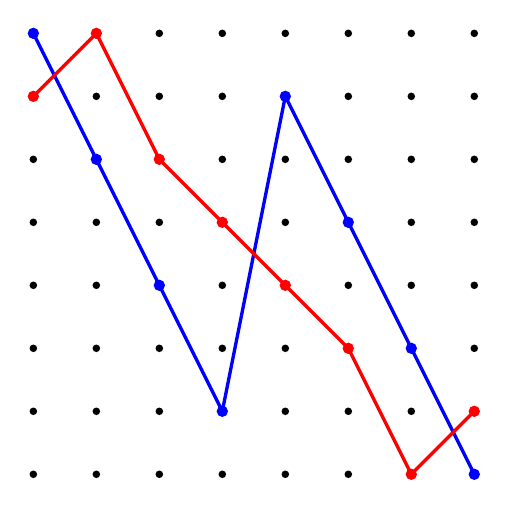
\begin{tikzpicture}[scale=0.8]

    % 1. Draw the 8x8 grid of black background dots
    \foreach \x in {1,...,8} {
        \foreach \y in {1,...,8} {
            \fill[black] (\x,\y) circle (0.06);
        }
    }

    % 2. Draw the blue path and its dots
    \draw[blue, very thick, line join=round, line cap=round] 
        plot coordinates {(1,8) (2,6) (3,4) (4,2) (5,7) (6,5) (7,3) (8,1)};
    
    \foreach \p in {(1,8), (2,6), (3,4), (4,2), (5,7), (6,5), (7,3), (8,1)} {
        \fill[blue] \p circle (0.09);
    }

    % 3. Draw the red path and its dots
    \draw[red, very thick, line join=round, line cap=round] 
        plot coordinates {(1,7) (2,8) (3,6) (4,5) (5,4) (6,3) (7,1) (8,2)};
    
    \foreach \p in {(1,7), (2,8), (3,6), (4,5), (5,4), (6,3), (7,1), (8,2)} {
        \fill[red] \p circle (0.09);
    }

\end{tikzpicture}

\caption{Visualization of the two permutation paths on an $8 \times 8$ grid.}
\end{figure}

% 3. Put this command exactly where you want your references list to appear (usually at the very end)
\printbibliography


\end{document}

